\clearpage\null\vfill
\thispagestyle{empty}
\begin{minipage}[b]{.9\textwidth}
  \begin{center}
  \setlength{\parskip}{.5\baselineskip}
  {\color{phdcol0}%
   \ccLogo\hspace{.1cm}%
   \ccAttribution\hspace{.1cm}%
   \ccNonCommercial\hspace{.1cm}%
   \ccNoDerivatives}\hspace{.15cm}%
  \footnotesize%
  This work is licensed under {\color{phdcol1}\textbf{http://creativecommons.org/licenses/by-nc-nd/3.0/}}
  \end{center}
\end{minipage}
\vspace*{2\baselineskip}

\clearpage

\thispagestyle{empty}
\vspace*{\stretch{1}}
\begin{flushright}
  \textit{Ah, la thèse.}
\end{flushright}
\vspace*{\stretch{7}}
%
%%
%\chapter*{Remerciements}
%
%
%\`A tous, \textbf{merci infiniment} !

%
\chapter*{Résumé Long}


Cette thèse traite la résolution du problème de satisfaisabilité booléenne (SAT).
Le problème de satisfabilité est un problème important qui traitent de problèmes importants dans différent domaines tel 
que la décision de planification~\cite{planning_92}, la biologie~\cite{biology_06}, la vérification de logiciel et de 
matériel informatique~\cite{biere1999symbolic}, de raisonnement automatique~\cite{heule2016solving}.
Leurs évolutions au cours des dernières décennies leurs ont permis de traiter des problèmes de plus en plus complexe.
Dans un travail récent, des chercheurs ont réussi a prouver à l'aide d'un solveur SAT, une borne maximum
pour le problème de coloration des triplets Pythagoriciens~\cite{heule2016solving}, avec une preuve de 200 TB.


Le principe de base de SAT est de déterminer si une formule propositionnelle
est satisfaisable, c'est à dire toutes les contraintes peuvent être satisfaites,
ou insatisfaisable, c'est à dire il n'y a aucun moyen de satisfaire toutes les contraintes avec une même affectation.
Ce calcul est effectué par un solveur SAT qui répond usuellement $\sat$ lorsque la formule est satisfaisable et $\unsat$ dans le cas
contraire.
Le problème SAT a été le premier problème à avoir été prouvé NP-Complet. Cela signifie que
l'on ne connaît pas d'algorithme capable de résoudre le problème avec une complexité polynomiale.
La résolution du problème est l'un des sept prix du millénaire, à savoir P = NP.


Malgré cette complexité, les solveurs SAT sont capables de résoudre de plus en plus de problème complexe.
Ce succès vient de l'introduction de différentes heuristiques sophistiquées et de l'optimisation de l'algorithme de
résolution des conflits appelé $\guillemotleft$ Conflict Driven Clause Learning$\guillemotright$ (CDCL) qui est basé sur le premier
algorithme (avec une utilisation non intensif de la  mémoire) nommé par ses auteurs Davis, Putnam, Logemann
et Loveland (DPLL)\cite{dpll_62}.


Cette algorithme peut être vu sous forme de l'exploration d'un arbre ou chaque branche représente 
une affectation. Il y a donc au total $2^n$ branches, avec $n$ le nombre de variables du problèmes.
Le principe de cet algorithme est d'explorer cet arbre binaire. 
La première étape consiste à choisir une variable dite de décision avec une polarité qui permet l'exploration
de l'arbre de recherche. Puis, d'effectuer les déductions logiques à partir de l'affection. 
Si l'algorithme découvre un conflit, c'est à dire que l'affectation courante n'est pas capable de satisfaire au moins une contrainte du problème, l'algorithme va calculé une clause dite de conflit qui permet d'élaguer 
cet espace de recherche qui ne contient pas de solution. Cette clause est une information redondante par
rapport au problème initial. Si aucun conflit n'est présent, l'algorithme choisit à nouveau une variable de décision. L'algorithme termine lorsque soit toutes les variables sont affecté au quel cas le problème 
est satisfait, soit un conflit est apparu avec uniquement des diductions logiques au quel cas le
problème est non satisfaisant.
La Figure~\ref{fig:cdclflow} présente sous forme d'un organigramme le fonctionnement de l'algorithme CDCL.


\begin{figure}[!htbp]
\begin{tikzpicture}[node distance=1.5cm,
,every node/.style={scale=0.7,fill=white, font=\sffamily}, align=center]
% Specification of nodes (position, etc.)
\tikzset{%	
	>={Latex[width=2mm,length=2mm]},
	% Specifications for style of nodes:
	base/.style = {rectangle, rounded corners, draw=black,
		minimum width=2cm, minimum height=1cm,
		text centered, font=\sffamily},
	question/.style = {base, diamond, fill=blue!15},
	unsat/.style = {base, fill=red!30,minimum width=3cm},
	sat/.style = {base, fill=green!30,minimum width=3cm},
	process/.style = {base, minimum width=2.5cm, fill=orange!15,
		font=\ttfamily},
}
\node (isfin) [question] {Variables toutes \\assignées ?};
\node (dec)     [process, below = of isfin]          {Choix variable \\ de decision};
\node (sdec)     [right = of dec]          {};
\node (idec) [left = of isfin]  {};
\node (prop)    [process, below = of dec ]          {Propagation unitaire};
\node (conf)    [question, below = of prop] { Conflit ?};
\node (confanalyse) [process, below = of conf] {Analyse du \\ conflit};
\node (learn) [process] at ($(prop) + (160pt, 0)$) {Apprentissage de la \\ clause de conflit};
\node (isend) [question] at ($(confanalyse) + (160pt, 0)$) {Niveau de \\decision zero ?};
\node (end) [unsat] at ($(isend) + (140pt, 0)$) {$\unsat$};
\node (ends) [sat] at ($(isfin) + (+160pt, 0)$){$\sat$};


\draw[->, thick]     (sdec) -- (dec);
\draw[->, thick]     (dec) -- (prop);
\draw[->, thick]     (prop) -- (conf);
\draw[->, thick]     (conf) -| node [yshift=5.5 cm] {non}(idec.center) -- (isfin);
\draw[->, thick]     (conf) -- node {oui} (confanalyse);
\draw[->, thick]     (isfin) -- node {non}(dec);
\draw[->, thick]     (confanalyse) --(isend);
\draw[->, thick]     (isend) -- node {oui}(end);
\draw[->, thick]     (isfin) -- node {oui}(ends);
\draw[->, thick]     (learn) -- (prop);
\draw[->, thick]     (isend) -- node [] {non}(learn);

\end{tikzpicture}
\caption{Organigramme de l'algorithme CDCL}
\label{fig:cdclflow}
\end{figure}

%\begin{figure}[!htbp]
%	\begin{tikzpicture}[node distance=1.5cm,
%	,every node/.style={scale=0.7,fill=white, font=\sffamily}, align=center]
%	% Specification of nodes (position, etc.)
%	\tikzset{%	
%		>={Latex[width=2mm,length=2mm]},
%		% Specifications for style of nodes:
%		base/.style = {rectangle, rounded corners, draw=black,
%			minimum width=2cm, minimum height=1cm,
%			text centered, font=\sffamily},
%		question/.style = {base, diamond, fill=blue!15},
%		unsat/.style = {base, fill=red!30,minimum width=3cm},
%		sat/.style = {base, fill=green!30,minimum width=3cm},
%		process/.style = {base, minimum width=2.5cm, fill=orange!15,
%			font=\ttfamily},
%	}
%	\node (isfin) [question] {All vars\\ assign?};
%	\node (dec)     [process, below = of isfin]          {Choose decision var};
%	\node (sdec)     [right = of dec]          {};
%	\node (idec) [left = of isfin]  {};
%	\node (prop)    [process, below = of dec ]          {Unit Propagation};
%	\node (conf)    [question, below = of prop] { IsConflict?};
%	\node (confanalyse) [process, below = of conf] {Conflict Analysis};
%	\node (learn) [process] at ($(prop) + (160pt, 0)$) {Learn conflict clause};
%	\node (isend) [question] at ($(confanalyse) + (160pt, 0)$) {is level\\zero?};
%	\node (end) [unsat] at ($(isend) + (140pt, 0)$) {$\unsat$};
%	\node (ends) [sat] at ($(isfin) + (+160pt, 0)$){$\sat$};
%	
%	
%	\draw[->, thick]     (sdec) -- (dec);
%	\draw[->, thick]     (dec) -- (prop);
%	\draw[->, thick]     (prop) -- (conf);
%	\draw[->, thick]     (conf) -| node [yshift=5.5 cm] {no}(idec.center) -- (isfin);
%	\draw[->, thick]     (conf) -- node {yes} (confanalyse);
%	\draw[->, thick]     (isfin) -- node {no}(dec);
%	\draw[->, thick]     (confanalyse) --(isend);
%	\draw[->, thick]     (isend) -- node {yes}(end);
%	\draw[->, thick]     (isfin) -- node {yes}(ends);
%	\draw[->, thick]     (learn) -- (prop);
%	\draw[->, thick]     (isend) -- node [] {no}(learn);
%	
%	\end{tikzpicture}
%	\caption{Organigramme de l'algorithme CDCL}
%	\label{fig:cdclflow}
%\end{figure}


Cependant certains problème présente des symétries, certaines branches de l'espace de recherche 
sont donc équivalentes à la symétrie près. Prenons comme exemple le $\guillemotleft$problème des pigeons $\guillemotright$ dans lequel nous avons un ensemble de pigeons qui doivent êtres attribués à des nids différents. Dans ce problème il y a un nids de moins que le nombre de pigeons.
Le but de ce problème est de déterminer si il est possible d'attribuer un nid différent à chaque pigeon.
 La figure~\ref{fig:holefr} pressente un instance de ce problème.
 
 
 \begin{figure}[!htbp]
 	\centering
 	\begin{tikzpicture}[
 	start chain = going right,
 	node distance = 0pt,
 	AStyle/.style={draw, minimum width=2em, minimum height=2em, 
 		outer sep=0pt, on chain, fill=yellow!0!white}]
 	\node [AStyle] (1) {\huge\textcolor{gray}{\PHdove}};
 	\node [AStyle] (4) {\huge\textcolor{gray}{\PHdove}};
 	\node [AStyle] (5) {\huge\textcolor{gray}{\PHdove}};
 	\node [AStyle, draw] (6) {\huge\textcolor{gray}{\PHdove}};
 	\node [ minimum width=2em, minimum height=2em, 
 	outer sep=1pt, on chain] (7) {\huge\textcolor{gray}{\PHdove}};
 	\end{tikzpicture}
 	\caption{Représentation graphique d'une instance du problème des pigeons(5 pigeons, 4 nids)}
 	\label{fig:holefr}
 \end{figure}
 
 
Pour un humain, la réponse à ce problème est évidente, mais un solveur de l'état de l'art va parcourir toutes 
les combinaisons possibles de couples (pigeon, nid), cela le mène a une explosion combinatoire.
Pour cette raison, résoudre ce problème avec un solveur s'avère très chronophage et même impossible dans des temps raisonnable
pour un nombre de pigeons supérieur a environ 15.

%Cependant, certains problèmes possèdent un espace de recherche énorme et ne peuvent pas 
%être traité par un solveur SAT. Un exemple d'un tel problème peut être le problème de tournées de véhicules (VRP). 
%Il s'agit du service d'entreprise de livraison, dans lequel étant donné une flotte de véhicules basés dans un dépôt, ceux ci doivent faire des rondes entre des clients qui ont demandés chacun une certaine quantité de marchandises. Le circuit effectué par un véhicule pour la visite de tous les clients
%est appelé la tournée du véhicule. L'objectif est de trouver la tournée qui minimise les coûts de livraison (monétaire, distance, temps, ....).
%
%
%Dans le problème précédent, renommer l'ensemble de véhicules identiques nous donnera exactement le même problème. C'est ce qu'on appelle une symétrie.

De manière plus  général, une symétrie est une transformation qui laisse un objet (ou un aspect de l'objet) inchangé. Les symétries sont généralement définie comme une propriété syntaxique d'un problème lorsque leur présence est inhérente à l'encodage du problème.
Dans ce cas, une permutation des variables préservent la spécification originale du problème.
Dans le cas où les symétries sont indépendantes d'une représentation particulière du problème, il s'agit de symétries sémantiques.

La présence de symétrie dans un problème force l'algorithme de recherche à explorer en vain l'espace de recherche symétrique et entrave considérablement ses performances. La rupture de symétrie est une approche qui évite au solveur de visiter l'espace de recherche symétrique.

Pour pouvoir exploiter les symétries, la première étape consiste à les trouver. Dans le contexte de la satisfaction booléenne, la détection des symétries syntaxique se fait par tout d'abord par la transformation de la spécification en un graphe coloré et ensuite à l'application d'un outil d'automorphisme de graphe.
Différent outils traitent ce problème dans l'état de l'art tel que $\bliss$~\cite{JunttilaKaski:ALENEX2007}, $\saucy$~\cite{katebi2010symmetry}, ...


Lorsque les symétries sont obtenues à l'aide de ces outils, l'approche la plus courante pour les exploiter est d'utiliser une technique de rupture de symétrie statique. Celui ci consiste à prendre le problème symétrique en entrée et à produire une formule équivalente en éliminant les symétries présentes dans le problème.
Cette technique est dite statique car elle est effectué avant la résolution du problème SAT. 

Pour produire une formule équivalente sans présence de symétries, le problème est augmenté par des 
contraintes de rupture de  symétries (e $\guillemotleft$symmetry breaking predicates $\guillemotright$ sbp). Celles ci empêchent le solveur d'explorer l'espace de recherche symétrique. 
Autrement dit, si l'on considère notre exemple précédent avec les pigeons, le premier pigeon est attribué a un
exactement un nid, la symétrie est alors "cassé".

Plusieurs outils tels que $\shatter$~\cite{} et $\breakid$~\cite{} utilisent cette technique pour accélérer le calcul du solveur en présence de symétries.
En général, cette approche apporte de bon résultats dans différentes instances symétriques mais possède des défauts. Parmi cela nous pouvons cité le nombre de contraintes ajoutées qui peut être exponentielle par rapport à la taille du problème, ce qui a pour conséquence de ralentir l'algorithme principal du solveur.
De plus, étant donné que ce calcul est effectué avant le lancement du calcul du solveur, celui-ci ne peut pas différentier les contraintes originales du problème avec les contraintes de rupture de symétrie. Avec cette information, le solveur peut modifier ces heuristiques, ce qui peut augmenter ces performances.
Pour ces raisons, certains problèmes avec de nombreuses symétries ne peuvent pas être traités avec cette technique.

Une autre approche dite rupture de symétrie dynamique consiste à utiliser les symétries durant l'algorithme de recherche du solveur SAT, plus précisément à modifier son comportement pour exploiter les propriétés de symétrie du problème. Cette approche consiste à déduire des faits symétrique par rapport aux déductions effectués par le solveur. Lorsque ces faits sont ignorés le solveur va explorer en vain l'espace de recherche symétrique.
Ces déductions réduisent le nombre de décisions qui sont des suppositions du solveur qui sont choisit de 
manière heuristiques et augmentent le nombre de propagations qui sont les déductions logique faites par le solveur. En d'autres termes, cette approche transforme les suppositions du solveur en déductions logiques.
Différents outils utilisent cette approche, nous pouvons cité parmi cela \textit{Symmchaff}
qui exploite que certains type spécifique de symétries, \textit{Symmetry Propagation (SP)}, \textit{Symmetry Learning Scheme (SLS)}, \textit{Symmetry Explanation Learning (SEL)} qui ajoutent les symétrique des
clauses apprises pour permettre les déductions symétriques.
Étant donné que cette approche est dynamique, il est possible pour le solveur 
d'intégrer des heuristiques spécifiques ou encore de combiner les différentes technique de rupture de symétrie.


Cette thèse vise à améliorer l'existant et rendre les solveurs plus performants en présence de symétries et
propose différente contributions allant dans ce sens.  


Notre première contribution consiste à mimer le comportement de la rupture de symétrie statique mais 
opère dynamiquement, pendant l'exécution du solveur. On ajoute dans le solveur un composant de symétrie opportuniste qui va détecter que le solveur parcours un espace de recherche symétrique et va ajouter
une contrainte appelé $\guillemotleft$ effectective symmetry breaking predicate $\guillemotright$ qui va empêcher le solveur de rester dans
l'espace de recherche symétrique. Cette contrainte est dite effective car à l'inverse de l'approche 
de rupture de symétrie  statique la contraintes est forcément utilisé par le solveur. Aucune contrainte
inutile est inséré dans le solveur. Cela a pour conséquence de réduire le nombre de contrainte et donc 
ne ralentit pas les solveur.


Ce composant de symétrie est fournit sous forme d'une bibliothèque codé en C++ et se nomme $\libdsb$.
Elle peut s'interfacer avec n'importe quelle solveur de type CDCL. 
Nous l'avons interfacé avec un solveur de l'état de l'art nommé $\minisat$~\cite{een2003extensible}. Au total, l' intégration de $\libdsb$ ajoute environ 60 lignes de code 
et augmente de code de $\minisat$ de 3\%.
$\libdsb$ est open source fournit sous la licence GPLv3 et est disponible sur Github à l'adresse suivante: \url{https://github.com/lip6/cosy}.


Nous avons comparés les performances de notre approche avec le solveur $\minisat$
Les nombreuses expérimentations effectuées sur les instances symétrique de la SAT Competiton~\cite{jarvisalo2012international} sur les six dernière années nous démontre que notre approche est aussi performante que les approches de ruptures de symétries statiques.
La figure~\ref{fig:frcactus} nous montre les résultats obtenus par notre approche par rapport à l'état de l'art sous forme 
d'un cactus plot, l'axe des abscisses nous montre le nombre d'instance réussi par chacun des solveurs et sur l'axe des ordonné nous pouvons voir
le temps de calcul des solveurs. Comme nous pouvons le constater les résultats diffèrent avec l'utilisation de l'outil d'automorphisme de 
graphe $\saucy$ ou $\bliss$. La principale différence entre ces deux outils est le nombre de permutations obtenus. $\bliss$ nous donne plus
de permutations que $\saucy$. Cela permet a notre outil $\cdclsym$ qui est une intégration de notre bibliothèque dans $\minisat$, d'atteindre 
un nombre d'instances résolues de environ 780 alors que le deuxième meilleur outil $\breakid$ atteint un nombre d'instance résolue de environ 760.


\begin{figure}[!htbp]
	\centering
	\subfloat[with \saucy]{{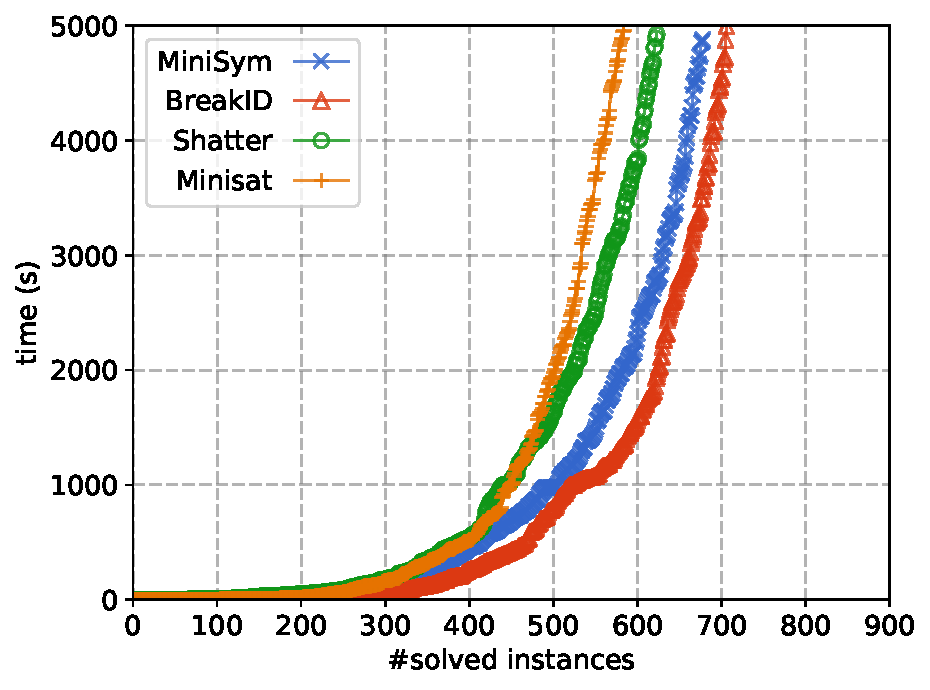
\includegraphics[scale=0.36]{img/saucy-result}}}%
	\qquad
	\subfloat[with \bliss]{{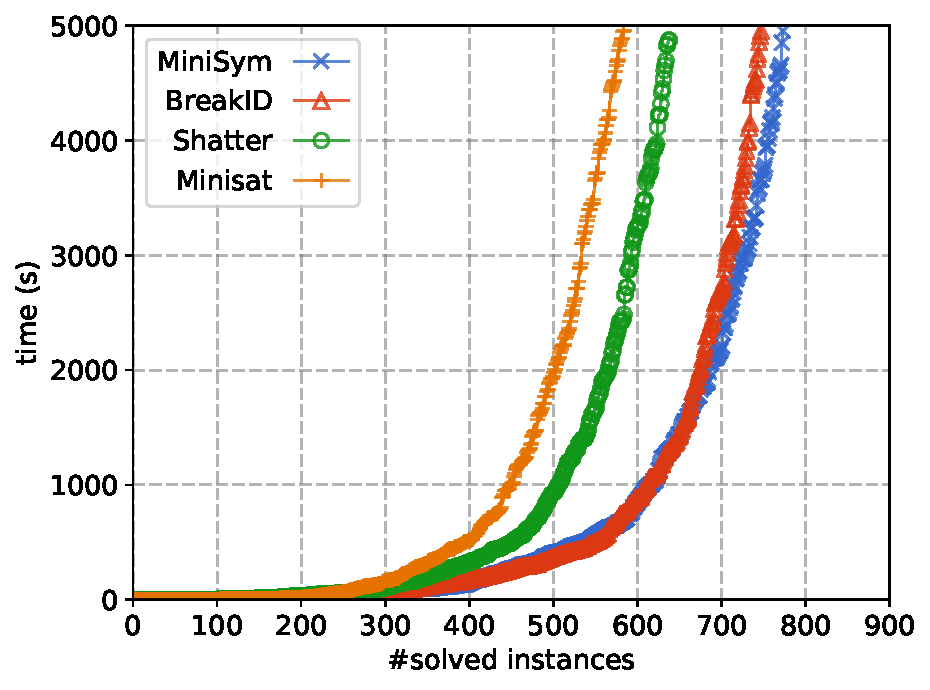
\includegraphics[scale=0.36]{img/bliss-result}}}%
	\caption{cactus plot  total number of instances}%
	\label{fig:frcactus}%
\end{figure}



Malgré les très bon résultats obtenue par notre approche certains problèmes qui sont résolue très 
rapidement par Symmetry Propagation (SP) ne peuvent pa être traité par notre approche et vise versa.
SP est une approche qui a pour but d'accélérer la traversé de l'espace de recherche en déduisant des faits symétrique 
à partir des déductions effectué par le solveur. A l'inverse notre approche consiste à éliminer les espaces de recherche 
symétriques. Ces deux approches sont donc orthogonales.
Notre deuxième contribution consiste à déterminer si cette combinaison est possible qui se résume donc à la question suivante:\\
Est il possible d'accélérer la traversé de l'espace de recherche tout en éliminant l'espace de symétrique ?

Pour que cette approche soit correcte, la contrainte qu'il faut absolument respecté est que la symétrie utilisé pour déduire les
faits symétriques doit être valide dans le problème actuel. Effectivement les clauses ajoutés pour éliminer l'espace de recherche
symétrique vont casser celle ci qui ne peuvent donc plus être utilisé pour propager les faits symétriques.
L'approche naïve qui consiste a enlever la symétrie dès lors qu'une contrainte de rupture de symétrie est ajouté mènerait très vite
à l'ensemble vide. Notre approche consiste a traqué les clauses utilisé et à connaître a tout instant l'ensemble des symétries
valide grâce à l'introduction dite de symétrie locale pour chaque clause.

Les expérimentations effectuées 


Pour cela différentes analyses théoriques et pratique ont dû être mis en place pour produire cette version
combiné qui bénéficie du meilleur des deux mondes.

\chapter*{Abstract}

This is an abstract.